\documentclass[conference]{IEEEtran}
\usepackage[authoryear,round]{natbib}
\usepackage[french]{babel}

\usepackage{amsmath,amssymb,amsfonts}
\usepackage{algorithmic}
\usepackage{graphicx}
\usepackage{textcomp}
\usepackage{comment}
\usepackage{xcolor}
\usepackage{tikz}
\usetikzlibrary{positioning,arrows.meta}

\setcitestyle{round,aysep={,},notesep={;}}
\def\BibTeX{{\rm B\kern-.05em{\sc i\kern-.025em b}\kern-.08em
    T\kern-.1667em\lower.7ex\hbox{E}\kern-.125emX}}

\begin{document}

\title{Utilisation des modèles de langages LLMs pour l’assistance dans les tâches en intelligence d’affaires}

\author{
\IEEEauthorblockN{WILHELMY Felix}
\IEEEauthorblockA{\textit{Département de génie LOG \& TI} \\
\textit{École de Technologie Supérieure}\\
Montréal, Canada \\
felix.wilhelmy.1@ens.etsmtl.ca}
\and
\IEEEauthorblockN{NOUBISSI KOM Carmen Wilfred}
\IEEEauthorblockA{\textit{Département de génie LOG \& TI} \\
\textit{École de Technologie Supérieure}\\
Montréal, Canada \\
carmen-wilfred.noubissi-kom.1@ens.etsmtl.ca}
\and
\IEEEauthorblockN{LAAZIRI Othman}
\IEEEauthorblockA{\textit{Département de génie LOG \& TI} \\
\textit{École de Technologie Supérieure}\\
Montréal, Canada \\
Othman.laaziri.1@ens.etsmtl.ca}
}

\maketitle

\begin{abstract}
Les systèmes d’intelligence d’affaires (\textit{Business Intelligence}, BI) sont essentiels aux organisations modernes pour transformer de grandes quantités de données en informations exploitables facilitant la prise de décisions stratégiques. Cependant, les méthodes traditionnelles de BI peinent à gérer efficacement la complexité et l’évolution constante des besoins organisationnels. Cet article examine comment les récents progrès en intelligence artificielle (IA), et en particulier les modèles de langage (\textit{Large Language Models}, LLMs), peuvent répondre à ces défis. Dans notre discussion, nous proposons un prototype de système qui utilise ces technologies et qui est adapté aux besoins spécifiques de l’entreprise Forester Inc.
\end{abstract}

\begin{IEEEkeywords}
intelligence artificielle, intelligence d’affaires, \textit{Large Language Models}
\end{IEEEkeywords}

\section{Introduction}
\label{sec:introduction}

Fondée en 1950 dans le sud du Québec, \textbf{Forester} est une entreprise commerciale diversifiée active dans la vente de matériel informatique et industriel ainsi que dans l’édition et la commercialisation de solutions logicielles. Confrontée à un environnement concurrentiel croissant, elle souhaite accroître son efficacité opérationnelle, fluidifier sa communication interne et externe, et améliorer la satisfaction de ses employés comme de ses clients. Ses priorités sont de répondre rapidement et précisément aux demandes, d’automatiser les tâches répétitives, de garantir un support continu (24/7) et d’optimiser la gestion de l’information afin d’identifier plus finement les opportunités et les risques stratégiques.

Les systèmes traditionnels d’intelligence d’affaires, bien qu’indispensables pour convertir d’importants volumes de données en informations exploitables, souffrent de délais élevés, d’une forte dépendance vis-à-vis des équipes techniques et d’une flexibilité limitée face à l’évolution rapide des besoins métiers. Les modèles de langage de grande taille (\textit{Large Language Models}, LLMs) constituent aujourd’hui un levier pour simplifier la génération de requêtes analytiques, accélérer la prise de décision et donner davantage d’autonomie aux utilisateurs non spécialistes.

\subsection{Structure de la revue}  
Cet article propose une revue de littérature structurée sur l’intégration des LLMs dans les systèmes de BI au moyen d’interfaces conversationnelles. Deux systèmes étudier servent de fil conducteur : \textbf{SiriusBI}, orienté vers l’échange en langage naturel multitours et donc particulièrement adapté aux utilisateurs non techniques, et \textbf{AutoBIR}, centré sur la rigueur technique grâce à la génération automatisée de requêtes NL2SQL, aux tests unitaires et à la boucle de correction automatique. Après avoir exposé les concepts fondamentaux de la BI classique et des LLMs en section \ref{sec:concepts_fondamentaux}. La section \ref{sec:chatbi} présentera ensuite le fonctionnement d'un assistant BI conversationnel (\emph{ChatBI}) et l'architecture d'un tel système adaptée aux besoins de Forester, tandis que la section \ref{sec:cas_etudes} détaillera les résultats et comparera SiriusBI et AutoBIR. Enfin, la section \ref{sec:conclusion} conclura et discutera les perspectives d’extensions, notamment l’ajout de modules de \textit{forecasting} et d’analyses prédictives.

\subsection{Méthodologie de rédaction}  
Dans le cadre d’une recherche exploratoire rapide, nous avons interrogé \textit{arXiv} et \textit{IEEE Xplore} avec les mots-clés « Large Language Models », « Business Intelligence », « NL2SQL » et « ChatBI », sans autre filtre. Deux articles applicatifs se sont immédiatement démarqués: SiriusBI \citep{jiang2024siriusbi} et AutoBIR \citep{busany2024autobir}. Pour étayer l’analyse, trois références techniques ont été ajoutées : l’article fondateur sur les Transformers \citep{vaswani2023attentionneed}, une synthèse sur les LLMs \citep{minaee2025llmsurvey}, et une étude sur les chatbots en contexte professionnel \citep{toxtli2018chatbot}. Ce corpus restreint de cinq articles constitue la base critique de la présente revue. 

\section{Concepts fondamentaux}
\label{sec:concepts_fondamentaux}

\subsection{Intelligence d’affaires : des données aux décisions}

L’intelligence d’affaires regroupe les méthodes, outils et pratiques visant à collecter, stocker, analyser et présenter des données pour aider à la prise de décision. Un système BI classique se compose généralement des étapes suivantes :
\begin{enumerate}
    \item \textbf{Extraction et intégration} des données (ETL) depuis des sources variées (bases de données relationnelles, fichiers, ERP, CRM, etc.) ;
    \item \textbf{Stockage} des données dans un entrepôt ou un data lake ;
    \item \textbf{Modélisation} et agrégation des données pour créer des indicateurs clés de performance (KPI) ;
    \item \textbf{Analyse} via des requêtes SQL, des scripts analytiques (Python, R) ou des solutions de BI (tableaux de bord, rapports, cubes OLAP) ;
    \item \textbf{Restitution} sous forme de tableaux de bord, graphiques interactifs ou rapports automatisés pour les décideurs.
\end{enumerate}

Ces étapes requièrent souvent un certain niveau d’expertise technique : il faut savoir rédiger des requêtes complexes, comprendre la structure des entrepôts de données et interpréter les résultats. Par conséquent, les utilisateurs métiers (non-développeurs) ont tendance à dépendre des équipes techniques pour formuler des analyses, ce qui engendre des délais et des risques de mauvaise interprétation.

\subsection{Les modèles de langage (LLMs)}
\label{sec:utilisation_llms}

La modélisation du langage, ou \textit{Natural Language Processing} (NLP), est étudiée depuis plus de sept décennies, notamment depuis les travaux pionniers de Shannon (1950) sur l’application de la théorie de l’information au langage humain.

Les progrès majeurs récents proviennent des \textit{Large Language Models} (LLMs) fondés sur l’architecture \textit{Transformer} introduite par \citet{vaswani2023attentionneed}. Entraînés à l’échelle du Web, ces modèles (exp. \textit{GPT-4}, \textit{PaLM} et \textit{LLaMA}) repoussent les limites du raisonnement séquentiel et alimentent déjà des outils grand public comme \textit{ChatGPT} ou \textit{Microsoft Copilot}, capables de suivre des instructions complexes et d’enchaîner plusieurs étapes de raisonnement. Les différences de qualité entre LLMs proviennent alors (i) de la taille du modèle (nombre de paramètres), (ii) du volume de données pré-entraînées et (iii) des stratégies de spécialisation (\emph{instruction\,tuning}, RAG, RLHF, etc.).

Cette section présente, sans entrer dans les détails, les deux idées clés qui sous-tendent leur efficacité.

\begin{enumerate}
    \item \textbf{Représentations distribuées} : chaque mot, nombre ou symbole est projeté dans un espace vectoriel dense (typiquement $d_{\text{model}} \in [10^3,10^4]$), ce qui capture sa sémantique sous forme compacte ;
    \item \textbf{Attention multi-têtes} : le modèle pondère simultanément plusieurs relations internes à la séquence pour identifier les tokens les plus pertinents.
\end{enumerate}

Le coeur du calcul est l’opération d’attention :
\begin{equation}
\mathrm{Attention}(Q,K,V)=\mathrm{softmax}
      \!\bigl(\tfrac{QK^{\top}}{\sqrt{d_k}}\bigr)\,V,
\end{equation}
\noindent où $Q$, $K$ et $V$ sont respectivement les matrices de \emph{queries}, \emph{keys} et \emph{values} obtenues par projection linéaire des embeddings, et $d_k$ est la dimension au numérateur qui normalise la variance.

\begin{figure}[ht]
    \centering
    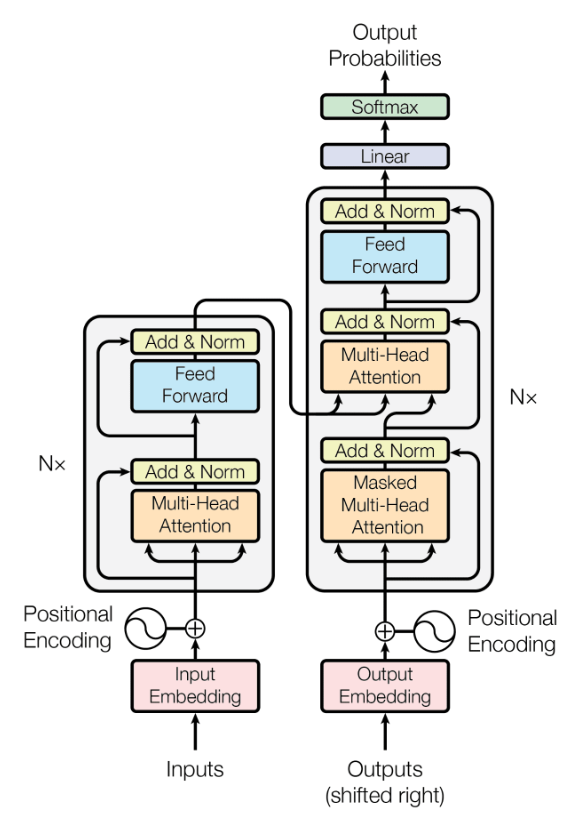
\includegraphics[width=1\linewidth]{figures/transformer.png}
    \caption{Architecture d’un Transformer. À gauche, l’encodeur empile des blocs « attention multi-têtes + réseau feed-forward », chacun entouré d’une connexion résiduelle et d’une normalisation de couche. À droite, le décodeur reprend la même structure, ajoute une attention croisée vers la sortie de l’encodeur et applique un masque causal garantissant que la prédiction à la position $i$ ne dépend que des positions $<i$.}
    \label{fig:transformer-architecture}
\end{figure}

\section{Assistant BI Conversationnel (ChatBI)}
\label{sec:chatbi}

Les sections précédentes ont présenté, d’une part, les bases de l’intelligence d’affaires (BI) — du pipeline \textit{ETL} à la restitution visuelle — et, d’autre part, les principes des modèles de langage de grande taille (LLMs).  Nous disposons donc, d’un côté, d’un vaste écosystème d’outils capables d’extraire la valeur de données hétérogènes ; de l’autre, d’algorithmes conversationnels capables de raisonner sur un corpus étendu de connaissances.  La rencontre de ces deux mondes façonne une nouvelle génération de plateformes : les \textbf{assistants BI conversationnels}, ou \emph{ChatBI}, qui promettent d’abaisser la barrière technique séparant les utilisateurs métiers de leur patrimoine informationnel.

\subsection{Offrir une interface adaptée à tous les profils}
\label{sec:interface_profiles}

Une interface bien conçue favorise l’adoption : elle doit permettre à des utilisateurs de différents niveaux d’interagir efficacement avec l’outil selon leurs besoins. Que ce soit via une interface unifiée ou intégrée dans des environnements existants (notebooks, outils de BI), l’objectif est de réduire la friction, accompagner l’utilisateur et faciliter la collaboration.

\subsection{Compréhension et analyse des données}
\label{sec:comprehension_donnees}

Pour un \emph{ChatBI} (évolution du système BI traditionnel vers un système capable de comprendre des requêtes sous forme de langage naturel~\citep{jiang2024siriusbi}), il ne suffit pas de connaître le langage naturel : il faut aussi savoir connecter la requête d’un utilisateur aux données de l’entreprise. Cela demande une connaissance de la structure, des indicateurs utilisés et de leur interprétation. Il est également crucial d’avoir un système agnostique capable d’agréger différentes sources de données.

Plusieurs approches récentes, comme celle de Jiang et al. (2024)~\citep{jiang2024siriusbi} dans le système SiriusBI, montrent l’intérêt de créer un graphe de connaissances qui rassemble ces informations à partir de sources internes (bases de données, scripts SQL/Python, dictionnaires métier). Ce graphe guide alors le modèle pour qu’il interprète correctement les questions, même si elles sont formulées de façon floue ou incomplète.

\subsubsection{Structurer les échanges entre modules}

Une solution BI performante repose sur un enchaînement de modules spécialisés : analyse de la requête en \textit{Natural Language Processing}, génération de code (SQL ou Python), exécution sur la base de données, puis restitution visuelle ou textuelle.

SiriusBI \citep{jiang2024siriusbi} applique ce principe avec son module MRD-Q qui dialogue, publie l’intention clarifiée sur le bus, puis attend que le module SQL confirme l’exécution.  AutoBIR \citep{busany2024autobir} adopte un schéma similaire mais ajoute un canal « tests unitaires » pour la boucle de correction automatique.

\subsection{Architecture d’un système ChatBI}
\label{sec:architecture_chatbi}

Un système ChatBI repose sur quatre modules interdépendants qui transforment une requête en langage naturel en analyses exploitables. Le \emph{Module de dialogue} établit et maintient la conversation, clarifie les intentions et s’assure que la demande est complète. Le \emph{Module de génération de requêtes} traduit cette intention en requêtes SQL (ou équivalent) conformes aux schémas et règles de l’entreprise. Le \emph{Module Insight} exécute ces requêtes, produit les artefacts attendus (visualisations, rapports, statistiques) et offre des analyses complémentaires. Enfin, la \emph{Base de connaissances} centralise toutes les métadonnées, définitions métier et règles de sécurité permettant de guider les autres modules et de garantir la validité des résultats.

\begin{figure*}[t]
    \centering
    \begin{tikzpicture}[
        node distance=2cm,
        >={Triangle[length=4pt,width=3pt]},
        box/.style={draw, rectangle, minimum width=3cm, minimum height=1.2cm, align=center},
        smallbox/.style={draw, rectangle, minimum width=1.5cm, minimum height=1.2cm, align=center}
    ]
    % Nœuds
    \node[box] (user) at (0,4)      {Utilisateur};
    \node[box] (dialogue) at (10,4) {Module de dialogue};
    \node[box] (kb) at (5,2)        {Base de connaissances};
    \node[box] (query) at (10,0)    {Module de requêtes};
    \node[box] (insight) at (0,0)   {Module Insight};
    \node[smallbox] (data) at (14,0) {Sources de données};

    % Flèches
    \draw[->] ([yshift=10pt]user.east) to node[above] {Interroger} ([yshift=10pt]dialogue.west);
    \draw[->] ([yshift=-10pt]dialogue.west) to node[below] {Précisions} ([yshift=-10pt]user.east);
    \draw[->] ([xshift=8pt]dialogue.south) -- node[right] {Intention} ([xshift=8pt]query.north);
    \draw[<->, bend right=15] ([yshift=5pt]kb.east) to node[midway,above] {Contexte} (dialogue.south);
    \draw[->, bend left=15] ([yshift=-5pt]kb.east) to node[midway,below] {Définitions} (query.north);
    \draw[->, bend right=15] ([yshift=-5pt]kb.west) to node[midway,below] {Définitions} (insight.north);
    \draw[<->] (query) -- node[midway,above] {SQL} (data);
    \draw[->] (query) to node[above] {Data Bindings} (insight.east);
    \draw[->] ([xshift=-8pt]insight.north) to node[right] {Artefacts} ([xshift=-8pt]user.south);
    \end{tikzpicture}
    \caption{Architecture générale d’un système ChatBI. L’utilisateur saisit sa requête en langage naturel, que le Module de dialogue reformule et clarifie avant de la transmettre au Module de génération de requêtes. Ce dernier interagit avec la Base de connaissances pour construire des requêtes SQL conformes. Les Sources de données fournissent les résultats, que le Module Insight transforme en visualisations ou rapports visibles par l’utilisateur.}
    \label{fig:chatbi-architecture}
\end{figure*}

\subsubsection{Module de dialogue}
Ce module reçoit la requête en langage naturel et entame un dialogue en plusieurs étapes afin de vérifier la syntaxe, détecter les entités métier (dimensions, indicateurs) et compléter les informations à partir de l’historique. Si un détail manque, il interroge l’utilisateur. Ensuite, il consulte la base de connaissances pour valider les termes métier (tables, champs, synonymes). Enfin, il synthétise la requête interprétée et la soumet à l’utilisateur pour confirmation. Cette approche garantit la précision de l’intention sans exiger de compétences techniques.

\subsubsection{Module de requêtes}
Une fois l’intention validée, ce module identifie les tables et jointures nécessaires via la base de connaissances, puis construit la requête SQL (ou API équivalente) selon les conventions internes. Pour assurer la fiabilité, il crée des tests unitaires. Si un test échoue, la requête est ajustée et retestée jusqu’à obtenir un résultat cohérent. En mode supervisé, l’utilisateur peut valider chaque étape (sélection des tables, filtres, structure de la requête) avant exécution.

\subsubsection{Module Insight}
Après exécution, ce module récupère les résultats bruts pour produire :
\begin{itemize}
    \item des \emph{visualisations} : graphiques, tableaux de bord ;
    \item des \emph{rapports analytiques} : résumés textuels, PDF, exports ;
    \item d’autres \emph{livrables} : CSV, modèles statistiques, etc.
\end{itemize}
L’utilisateur visualise d’abord une version préliminaire, puis peut demander des ajustements (changement de graphique, affinement de filtres, analyses complémentaires). Le processus peut alors repartir d’un nouveau dialogue pour affiner le paramétrage.

\subsubsection{Base de connaissances et modélisation}
Dans un contexte réel, une application BI requiert une quantité considérable d’informations propres au domaine concerné. Pour fonctionner correctement, un LLM doit comprendre cette structure, les règles et les indicateurs spécifiques à l’organisation. La base de connaissances est le référentiel central : un \emph{graphe de connaissances} relie les tables physiques aux définitions logiques (termes métier, abréviations, relations hiérarchiques). Elle contient également :
\begin{itemize}
    \item le \emph{glossaire métier} : définitions des indicateurs clés et synonymes internes ;
    \item les \emph{métadonnées techniques} : schémas, types, contraintes, règles d’accès.
\end{itemize}
Ce référentiel permet de traduire une requête naturelle en entités de la base de données, d’éviter les ambiguïtés et de guider chaque module dans la génération et l’exécution des requêtes.


\subsection{Intégrer les spécificités du domaine}

Dans un contexte réel, une application BI requiert une quantité considérable d’informations propres au domaine concerné. Pour fonctionner correctement, un LLM doit comprendre la structure, les règles et les indicateurs spécifiques à l’organisation.

\subsection{Gestion de la cohérence des résultats}

La cohérence des réponses d’un ChatBI est cruciale et loin d’être garantie. Plusieurs techniques ont été proposées pour améliorer cet aspect :
\begin{itemize}
    \item Utilisation d’un historique conversationnel~\citep{jiang2024siriusbi}, ce qui permet au ChatBI d’améliorer grandement sa compréhension du domaine et des requêtes antérieures de l’entreprise ;
    \item Techniques d’apprentissage auto-supervisées via des systèmes de correction du code généré par le système~\citep{busany2024autobir} ;
    \item Dépendance entre les cellules pour reconstruire le raisonnement analytique.
\end{itemize}

Une stratégie mixte selon le mode d’interaction (conversationnel ou code) pourrait offrir davantage de robustesse.


\subsection{Sécurité opérationnelle}

L’isolement des \textit{credentials}, le chiffrage des connexions (\textit{TLS}) et la vérification systématique des droits SQL (\texttt{row-level security}) s’imposent pour empêcher qu’une requête générée par le LLM n’exfiltre des données sensibles.  Des mécanismes d’obfuscation ou de \textit{data masking} peuvent être injectés automatiquement dans la requête avant exécution \citep{busany2024autobir}.

\subsection{Gouvernance et éthique}

Au-delà de la sécurité technique, la gouvernance des données est un grand enjeux. Au Québec, la loi 25 impose une gestion rigoureuse des renseignements personnels. Les journaux de conversation, données et tous autres artéfacts doivent donc être anonymisés et archivés selon un calendrier légalement défini. 

\begin{figure*}
    \centering
    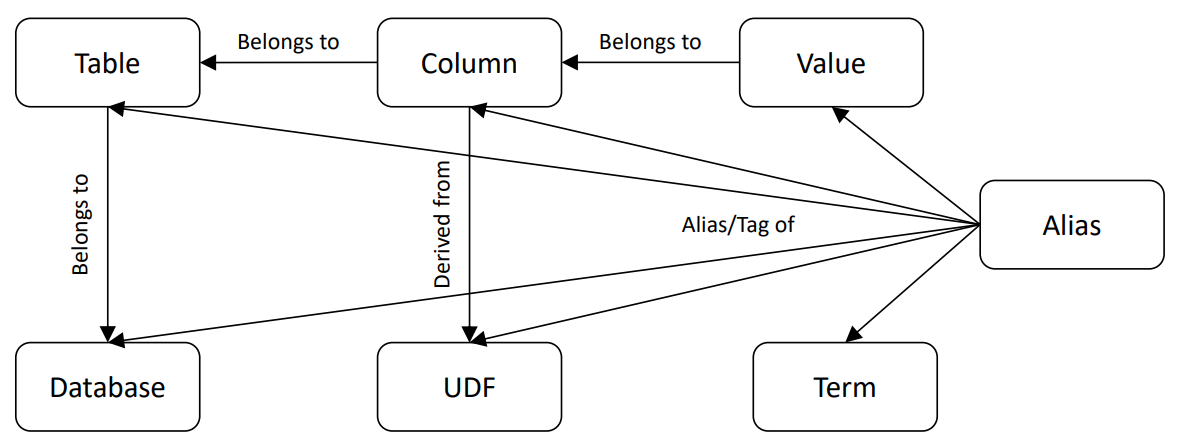
\includegraphics[width=0.48\textwidth]{figures/knowledge_graph.png} \hfill
    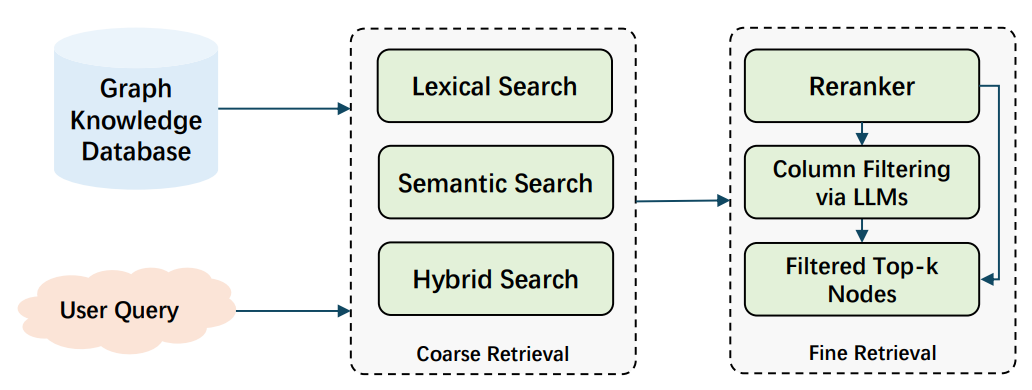
\includegraphics[width=0.48\textwidth]{figures/knowledge_retreival.png}
    \caption{Intégration des connaissances et recherche dans un système BI assisté par LLM. \emph{À gauche}, le \textit{graphe de connaissances (Knowledge Graph)} organise les tables physiques, les définitions métier et les relations sémantiques sous forme de triplets (nœuds = entités, arêtes = relations). \emph{À droite}, le module de recherche assisté par LLM interroge ce graphe pour formuler, raffiner et valider des requêtes en langage naturel, en combinant la précision factuelle du graphe et la générativité du LLM pour améliorer la pertinence des réponses.}
    \label{fig:knowledge-components}
\end{figure*}

\section{Études de cas et résultats observés}
\label{sec:cas_etudes}

Dans cette section, nous analysons deux travaux récents qui illustrent l’intégration de LLMs dans des environnements BI : \emph{SiriusBI} de \cite{jiang2024siriusbi} et \emph{AutoBIR} de \cite{busany2024autobir}. Pour les deux études, la métrique principale est l’\textbf{UEX} (\emph{Useful Execution Accuracy}), définie comme le pourcentage de requêtes générées pour lesquelles \emph{(i)} le SQL s’exécute sans erreur et \emph{(ii)} le résultat est jugé pertinent par rapport à l’intention métier \cite{jiang2024siriusbi}.  

\subsection{SiriusBI (Jiang \textit{et al.}, 2024)}

SiriusBI s’attaque au problème NL2SQL en contexte mono‐ et multi‐tour via un \emph{graphe de connaissances} qui décrit schémas et définitions métier et le module \emph{MRD-Q} (\textit{Multi-Round Dialogue with Querying}) pour clarifier la requête avant génération du SQL.

\begin{table}[ht]
\centering
\caption{Résultats de SiriusBI sur les jeux \textbf{SRD} (single-round) et \textbf{MRD} (multi-round) reportés par \citeauthor{jiang2024siriusbi} \citeyearpar{jiang2024siriusbi}.}
\label{tab:siriusbi-results}
\begin{tabular}{|l|c|c|}
\hline
\textbf{Variante} & \textbf{UEX SRD (\%)} & \textbf{UEX MRD (\%)}\\
\hline
DIN-SQL (baseline)          & 30,06 & 11,25 \\
MAC-SQL (baseline)          & 36,42 & 15,63 \\
MRD-SQL (fine-tuned)        & 61,85 & 28,13 \\
SiriusBI two-step           & 79,19 & 55,00 \\
\textbf{SiriusBI one-step}
& \textbf{83,24} 
& \textbf{62,50} \\
\hline
\end{tabular}
\end{table}

La version \emph{one-step} surpasse la baseline MRD-SQL de +21 pt sur SRD et +34 pt sur MRD, démontrant l’intérêt du couplage \textit{graphe + dialogue}.

\subsection{AutoBIR (Busany \textit{et al.}, 2024)}

AutoBIR propose un pipeline NL2SQL fondé sur une boucle de validation par tests unitaires :  
\begin{enumerate}
    \item génération initiale du SQL par LLM ;  
    \item exécution d’une suite de tests auto-générés ;  
    \item correction automatique jusqu’à validation complète.
\end{enumerate}

\begin{table}[ht]
\centering
\caption{Résultats AutoBIR sur \textit{AdventureWorks2014} rapportés par \citeauthor{busany2024autobir} \citeyearpar{busany2024autobir}.}
\label{tab:autobir-results}
\begin{tabular}{|l|c|}
\hline
\textbf{Métrique} & \textbf{Valeur} \\
\hline
Exact Match                & 85,3 \% \\
Execution Accuracy         & 88,7 \% \\
Test-Case Pass Rate        & 92,4 \% \\
Temps moyen de génération  & 1,8 s \\
\hline
\end{tabular}
\end{table}

La stratégie de tests réduit de 60 \% la consommation de tokens et augmente de 58 \% la précision finale, tout en offrant une garantie fonctionnelle avant exécution.

Bien que SiriusBI et AutoBIR reposent tous deux sur des LLMs pour traduire des requêtes en langage naturel en SQL, ils répondent à des priorités distinctes. SiriusBI, proposé par \citeauthor{jiang2024siriusbi}, met l’accent sur la compréhension conversationnelle: son module MRD-Q clarifie l’intention utilisateur au fil d’un dialogue multi-tour, tandis qu’un graphe de connaissances garantit la cohérence sémantique. Cette combinaison permet à la variante \emph{one-step} d’atteindre 62,5 \% d’UEX sur des dialogues multi-tours, dépassant de 34 points la meilleure ligne de base (MRD-SQL fine-tuned).

À l’inverse, AutoBIR, décrit par \citeauthor{busany2024autobir} \citeyearpar{busany2024autobir}, privilégie la robustesse et la validité du code généré. Après une première génération SQL, une suite de tests unitaires auto-produits vérifie l’exécution et la pertinence des résultats; les requêtes sont ensuite corrigées jusqu’à passer l’ensemble des tests. Cette stratégie offre 88,7 \% d’\emph{Execution Accuracy} et 92,4 \% de taux de succès aux tests sur le schéma AdventureWorks2014, tout en réduisant de 60 \% la consommation de tokens grâce à la boucle de correction.

Ainsi, SiriusBI se distingue par sa capacité à gérer des requêtes complexes et ambiguës via un dialogue riche, ce qui le rend particulièrement adapté aux contextes où la clarté métier prime. AutoBIR, de son côté, se révèle plus pertinent lorsque la priorité est de garantir la validité fonctionnelle avant exécution, notamment dans des environnements soumis à des contraintes de conformité ou de gouvernance des données. Les deux approches apparaissent donc complémentaires: la première optimise la compréhension sémantique, la seconde sécurise l’exécution, ouvrant la voie à des architectures hybrides combinant dialogue multi-tour et validation par tests unitaires.

\section{Conclusion}
\label{sec:conclusion}

Dans cette revue de littérature, nous avons montré que l’intégration des LLMs dans les systèmes BI permet de simplifier considérablement la génération de requêtes analytiques, d’accélérer la prise de décision et d’élargir l’autonomie des utilisateurs métiers. Les études de cas SiriusBI~\citep{jiang2024siriusbi} et AutoBIR~\citep{busany2024autobir} montrent qu’un pipeline structuré—du dialogue en langage naturel à la génération et à la validation automatique de code—peut atteindre une très bonne précision.

Au-delà de la simple agrégation de chiffres, un ChatBI pourrait également :
\begin{itemize}
    \item proposer des scénarios de \textit{forecasting} (budgétisation) en s’appuyant sur des modèles statistiques ou économétriques intégrés ;
    \item générer des analyses de corrélation ou de segmentation (\textit{k-means}, \textit{clustering}) pour identifier des comportements ou des segments de clients spécifiques ;
    \item interagir directement avec des modèles de \textit{machine learning} externes afin d’intégrer des recommandations prédictives dans le processus décisionnel.
\end{itemize}

Ces extensions ouvrent la voie à une BI plus proactive et prédictive, où le LLM ne se contente plus de traduire une requête, mais devient un catalyseur d’analyses avancées. En implémentant ces cas d’usage, on pourra mesurer l’impact sur la capacité à anticiper les tendances, à optimiser les budgets et à personnaliser les recommandations pour chaque unité métier de Forester Inc.

En conclusion, exploiter les LLMs pour l’assistance BI ne se limite pas à automatiser la génération de requêtes : c’est une véritable opportunité pour transformer les systèmes d’information en plateformes d’analyse dynamique et prédictive.

\cleardoublepage
\onecolumn
\bibliographystyle{bibETS}
\bibliography{biblio}


\end{document}